


\tikzset{every picture/.style={line width=0.75pt}} %set default line width to 0.75pt        

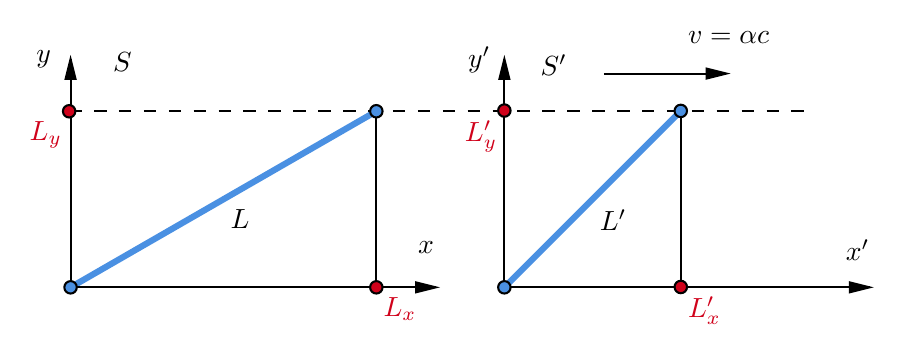
\begin{tikzpicture}[x=0.75pt,y=0.75pt,yscale=-1,xscale=1]
%uncomment if require: \path (0,159); %set diagram left start at 0, and has height of 159

%Straight Lines [id:da6456864463685883] 
\draw  [dash pattern={on 4.5pt off 4.5pt}]  (49.32,46.17) -- (407,46.17) ;
%Straight Lines [id:da6415604239700683] 
\draw [color={rgb, 255:red, 74; green, 144; blue, 226 }  ,draw opacity=1 ][line width=2.25]    (50,131) -- (197.32,46.17) ;
%Straight Lines [id:da6891479316334994] 
\draw [color={rgb, 255:red, 74; green, 144; blue, 226 }  ,draw opacity=1 ][line width=2.25]    (259,131) -- (344,46) ;
%Straight Lines [id:da21324392900197542] 
\draw    (50,131) -- (226,131) ;
\draw [shift={(228,131)}, rotate = 180] [fill={rgb, 255:red, 0; green, 0; blue, 0 }  ][line width=0.08]  [draw opacity=0] (12,-3) -- (0,0) -- (12,3) -- cycle    ;
%Straight Lines [id:da45941606825784165] 
\draw    (50,131) -- (50,21) ;
\draw [shift={(50,19)}, rotate = 90] [fill={rgb, 255:red, 0; green, 0; blue, 0 }  ][line width=0.08]  [draw opacity=0] (12,-3) -- (0,0) -- (12,3) -- cycle    ;
%Straight Lines [id:da6018132559816893] 
\draw    (259,131) -- (435,131) ;
\draw [shift={(437,131)}, rotate = 180] [fill={rgb, 255:red, 0; green, 0; blue, 0 }  ][line width=0.08]  [draw opacity=0] (12,-3) -- (0,0) -- (12,3) -- cycle    ;
%Straight Lines [id:da07174551591338907] 
\draw    (259,131) -- (259,21) ;
\draw [shift={(259,19)}, rotate = 90] [fill={rgb, 255:red, 0; green, 0; blue, 0 }  ][line width=0.08]  [draw opacity=0] (12,-3) -- (0,0) -- (12,3) -- cycle    ;
%Straight Lines [id:da28631990964329224] 
\draw    (197.32,46.17) -- (197.32,131) ;
%Straight Lines [id:da8474302302384931] 
\draw    (344,46) -- (344,130.83) ;
%Shape: Circle [id:dp6376135028535224] 
\draw  [color={rgb, 255:red, 0; green, 0; blue, 0 }  ,draw opacity=1 ][fill={rgb, 255:red, 208; green, 2; blue, 27 }  ,fill opacity=1 ] (194.32,131) .. controls (194.32,129.34) and (195.66,128) .. (197.32,128) .. controls (198.98,128) and (200.32,129.34) .. (200.32,131) .. controls (200.32,132.66) and (198.98,134) .. (197.32,134) .. controls (195.66,134) and (194.32,132.66) .. (194.32,131) -- cycle ;
%Shape: Circle [id:dp9795400606223699] 
\draw  [color={rgb, 255:red, 0; green, 0; blue, 0 }  ,draw opacity=1 ][fill={rgb, 255:red, 208; green, 2; blue, 27 }  ,fill opacity=1 ] (46.32,46.17) .. controls (46.32,44.51) and (47.66,43.17) .. (49.32,43.17) .. controls (50.98,43.17) and (52.32,44.51) .. (52.32,46.17) .. controls (52.32,47.82) and (50.98,49.17) .. (49.32,49.17) .. controls (47.66,49.17) and (46.32,47.82) .. (46.32,46.17) -- cycle ;
%Shape: Circle [id:dp7726188473166951] 
\draw  [color={rgb, 255:red, 0; green, 0; blue, 0 }  ,draw opacity=1 ][fill={rgb, 255:red, 74; green, 144; blue, 226 }  ,fill opacity=1 ] (194.32,46.17) .. controls (194.32,44.51) and (195.66,43.17) .. (197.32,43.17) .. controls (198.98,43.17) and (200.32,44.51) .. (200.32,46.17) .. controls (200.32,47.82) and (198.98,49.17) .. (197.32,49.17) .. controls (195.66,49.17) and (194.32,47.82) .. (194.32,46.17) -- cycle ;
%Shape: Circle [id:dp9274742345160407] 
\draw  [color={rgb, 255:red, 0; green, 0; blue, 0 }  ,draw opacity=1 ][fill={rgb, 255:red, 74; green, 144; blue, 226 }  ,fill opacity=1 ] (47,131) .. controls (47,129.34) and (48.34,128) .. (50,128) .. controls (51.66,128) and (53,129.34) .. (53,131) .. controls (53,132.66) and (51.66,134) .. (50,134) .. controls (48.34,134) and (47,132.66) .. (47,131) -- cycle ;
%Shape: Circle [id:dp49548641472371857] 
\draw  [color={rgb, 255:red, 0; green, 0; blue, 0 }  ,draw opacity=1 ][fill={rgb, 255:red, 74; green, 144; blue, 226 }  ,fill opacity=1 ] (256,131) .. controls (256,129.34) and (257.34,128) .. (259,128) .. controls (260.66,128) and (262,129.34) .. (262,131) .. controls (262,132.66) and (260.66,134) .. (259,134) .. controls (257.34,134) and (256,132.66) .. (256,131) -- cycle ;
%Shape: Circle [id:dp7855386744287358] 
\draw  [color={rgb, 255:red, 0; green, 0; blue, 0 }  ,draw opacity=1 ][fill={rgb, 255:red, 74; green, 144; blue, 226 }  ,fill opacity=1 ] (341,46) .. controls (341,44.34) and (342.34,43) .. (344,43) .. controls (345.66,43) and (347,44.34) .. (347,46) .. controls (347,47.66) and (345.66,49) .. (344,49) .. controls (342.34,49) and (341,47.66) .. (341,46) -- cycle ;
%Shape: Circle [id:dp08044621650283279] 
\draw  [color={rgb, 255:red, 0; green, 0; blue, 0 }  ,draw opacity=1 ][fill={rgb, 255:red, 208; green, 2; blue, 27 }  ,fill opacity=1 ] (341,130.83) .. controls (341,129.18) and (342.34,127.83) .. (344,127.83) .. controls (345.66,127.83) and (347,129.18) .. (347,130.83) .. controls (347,132.49) and (345.66,133.83) .. (344,133.83) .. controls (342.34,133.83) and (341,132.49) .. (341,130.83) -- cycle ;
%Shape: Circle [id:dp4552540178321567] 
\draw  [color={rgb, 255:red, 0; green, 0; blue, 0 }  ,draw opacity=1 ][fill={rgb, 255:red, 208; green, 2; blue, 27 }  ,fill opacity=1 ] (256,45.83) .. controls (256,44.18) and (257.34,42.83) .. (259,42.83) .. controls (260.66,42.83) and (262,44.18) .. (262,45.83) .. controls (262,47.49) and (260.66,48.83) .. (259,48.83) .. controls (257.34,48.83) and (256,47.49) .. (256,45.83) -- cycle ;
%Straight Lines [id:da031956449403815146] 
\draw    (307,28) -- (366,28) ;
\draw [shift={(368,28)}, rotate = 180] [fill={rgb, 255:red, 0; green, 0; blue, 0 }  ][line width=0.08]  [draw opacity=0] (12,-3) -- (0,0) -- (12,3) -- cycle    ;

% Text Node
\draw (216,107.4) node [anchor=north west][inner sep=0.75pt]    {$x$};
% Text Node
\draw (32,15.4) node [anchor=north west][inner sep=0.75pt]    {$y$};
% Text Node
\draw (240,13.4) node [anchor=north west][inner sep=0.75pt]    {$y'$};
% Text Node
\draw (422,106.4) node [anchor=north west][inner sep=0.75pt]    {$x'$};
% Text Node
\draw (275,17.4) node [anchor=north west][inner sep=0.75pt]    {$S'$};
% Text Node
\draw (69,16.4) node [anchor=north west][inner sep=0.75pt]    {$S$};
% Text Node
\draw (125.66,91.98) node [anchor=north west][inner sep=0.75pt]    {$L$};
% Text Node
\draw (303.5,91.9) node [anchor=north west][inner sep=0.75pt]    {$L'$};
% Text Node
\draw (346,134.23) node [anchor=north west][inner sep=0.75pt]  [color={rgb, 255:red, 208; green, 2; blue, 27 }  ,opacity=1 ]  {$L'_{x}$};
% Text Node
\draw (199.32,134.4) node [anchor=north west][inner sep=0.75pt]  [color={rgb, 255:red, 208; green, 2; blue, 27 }  ,opacity=1 ]  {$L_{x}$};
% Text Node
\draw (47.32,49.57) node [anchor=north east] [inner sep=0.75pt]  [color={rgb, 255:red, 208; green, 2; blue, 27 }  ,opacity=1 ]  {$L_{y}$};
% Text Node
\draw (257,49.23) node [anchor=north east] [inner sep=0.75pt]  [color={rgb, 255:red, 208; green, 2; blue, 27 }  ,opacity=1 ]  {$L'_{y}$};
% Text Node
\draw (346,6.4) node [anchor=north west][inner sep=0.75pt]    {$v=\alpha c$};


\end{tikzpicture}